\documentclass{article}
\usepackage{enumitem}
\usepackage{float}
\usepackage{graphicx}
\graphicspath{ {./design_images/} }

\usepackage[ddmmyyyy]{datetime}

\usepackage{hyperref} % allows for hyperlinks to be added to the document
\hypersetup{
    colorlinks,
    citecolor=black,
    filecolor=black,
    linkcolor=black,
    urlcolor=black,
    pdftitle={Research},
    pdfpagemode=FullScreen
}

\title{Engine Bravo Design}
\author{Sean Groenenboom \and Seger Sars \and Siem Vermeulen \and Angel Villanueva \and Ronan Vlak} % Sets authors name
\date{\today}

\begin{document}

\maketitle % Generates the title
\newpage

\tableofcontents
\newpage

\section{Abbreviations}
% Please make sure to keep this in alphabetical order!
\begin{tabular}{c|c}
  \textbf{Abbreviation} & \textbf{Full form}                \\ \hline
  API                   & Application programming interface \\ \hline
  SDL                   & Simple DirectMedia Layer          \\ \hline
  Hz                    & hertz                             \\ \hline
  Sfx                   & Sound effect(s)                   \\ \hline
  ECS                   & Entity Component System           \\ \hline
  UI                    & User interface                    \\
\end{tabular}

\section{Architecture}
The game engine is a singleton. This will be the only singleton in the engine.

Managers contain only references to the game objects which are relevant to them. For example, the physics manager only contains references to game objects with collider or rigidbody components.
Whenever a component is added to or removed from a game object, the game object calls a function in the game engine class. This adds the game object to an update queue. This update queue is used every cycle, where the engine checks all components of the object in the queue, and adds or removes them to the relevant managers.
\textbf{\textit{Motivate why we made this choice!}}

\subsection{GameObjects Architecture}
\begin{itemize}
    \item \textbf{GameObjects} are the main objects in the engine. They can contain multiple components, and are the objects which are updated every cycle.
    \item \textbf{Components} are the parts of the GameObjects. They can be added and removed from GameObjects, and are updated every cycle
\end{itemize}
ECS is not used because the decision was made that there is too little time to create a ECS system that is efficient enough to warrant the extra work it would cost to implement it.
Instead of ECS, a more standard Object Oriented approach is used.

Components can be added and removed from GameObjects at runtime. This is done by calling the addComponent and removeComponent functions of the GameObject class.
\section{UI}
\begin{itemize}
    \item \textbf{Three component types:} text, button, and image.
    \item \textbf{Text rendering:} font, text content, color, and transparency are adjustable.
    \item \textbf{Button:} has an interactable flag and an onclick callback.
    \item \textbf{Image:} has a sprite and a transparency value.
\end{itemize}

\noindent
There is a separate UI manager, which is responsible for checking where the clicks are, checking if the click was on a button, and calling the onclick callback if it was.
\section{Components}

Each component inherist from the Component class, which has a boolean to determine if the component is active.
\subsection{Transform}
Does not need an update flag when the position is changed, as a movable object is usually moving.

\subsection{Collider}
Has \texttt{bodyID}, which is needed for the physics.

\subsection{RigidBody}
Has \texttt{bodyID}, which is needed for the physics.

\subsection{Sprite}
Used to add a texture to a GameObject.

\subsection{IBehaviourScript}
IBehaviour script is an interface that can be used to create behaviour scripts for GameObjects.

\subsection{ParticleEmitter}
Used to create particle effects.

\subsection{AudioSource}
Used to add audio to a GameObject.

\section{Physics Update}
Physics are updated sequentially in the normal game loop.
The physics are updated at a fixed rate of 50 Hz. This is done by checking how much time has passed since the last physics update, and then updating the physics the required amount of times to keep up with the accumulated time.

\subsection{Alternatives Considered}
\begin{itemize}
    \item Updating physics using a deltatime. This is undesirable, because when the update frequency of the game drops, the physics will also slow down and become unreliable and prone to error.
    \item Multithreading. Not done because rendering can then copy old data and new data in a single frame. Alternative would be copying the data to physics and copying it back when physics is finished, but that would mean copying too much data back and forth per cycle.
\end{itemize}

\section{Physics Library}
Engine bravo makes use of the Box2D library to process any physics logic within the application. Box2D is chosen due to recommendations from teachers and since it is one of the only regularly updated ans accessible 2d physics libraries.

\section{Physics Object Types (in Box2D)}
\begin{itemize}
    \item \textbf{Staticbody}: objects which can be manually moved, but are not affected by gravity, mass, etc.
    \item \textbf{Kinematic body}: has zero mass, and can be moved by applying forces to it. It is not affected by gravity.
    \item \textbf{Dynamic body}: has mass, and is affected by gravity and other forces. It can be moved by applying forces to it.
\end{itemize}

\noindent
\textbf{Usage:}
\begin{itemize}
    \item \textbf{Staticbody} is used for walls, and objects which may move but only when explicitly told to do so.
    \item \textbf{Kinematic bodies} are not used, because the gravity of a dynamic body can instead be manually set to zero.
    \item \textbf{Dynamic bodies} are used for all objects which are affected by gravity and/or other forces.
\end{itemize}

\section{PhysicsEngine}{
  \begin{itemize}
      \item Steps are at 50 Hz
      \item substeps are configurable by the game programmer
      \item update method gets int of the amount of steps it need to set so less data gets copied to the world class
  \end{itemize}
 }
\section{Scene Manager}
\label{sec:sceneManager}
The SceneManager is responsible for creating, loading and unloading scenes.
It posses a list of scenes and keeps track of which scene is currently active.
To change the current scene the SceneManager can be addressed to load a new scene, which will happen after the current scene is rendered.
The SceneManager can also use the TileMap class to create a scene from a tilemap, which is described in more detail in the TileMaps chapter.

\subsection{Scene}
The Scene class is a container for GameObjects.
It has a list of GameObjects and a list of UIObjects.
The Scene class has functions to add and remove GameObjects and UIObjects.
The Scene class also has one or multiple cameras, which are used to render the scene.
The Camera is derived from the GameObject class, so it can be manipulated like any other GameObject.
The current Camera can be set, changed and retrieved from the Scene class.

\subsection{Camera}
The Camera class is derived from a GameObject that has a position and a size.
The size defined in the Camera class is the size of the view that is rendered.
The Camera class has a function to set the position of the camera, which will be used to render the scene.

\input{design_sections/tilemaps}
\section{Input}
\label{sec:input}
\subsection{Supported Input types}
\begin{itemize}
    \item \textbf{Keyboard input:} the engine supports all keys on the keyboard.
    \item \textbf{Mouse input:} the engine supports left, right, and middle mouse buttons.
    \item \textbf{Controller input:} the engine supports controller input, with analog values for the joysticks.
\end{itemize}

\subsection{Input class}
The input class is a singleton, and at the start of each cycle, it updates the input states.
This is done by checking the state of the input devices, and updating the input states accordingly.
After the input states are updated, the input class is responsible for checking if a key is pressed, released, or held down.
These calculations are done at the start of every cycle, and then the input states can be read from anywhere in the engine, but hopefully only used from the behavior scripts.

\subsection{Input contexts}
An input context is a state the input system can be in where it only allows certain inputs to go through.
For example, when the player is in the main menu, the input context is set to the main menu context, and only the inputs which are relevant to the main menu are allowed to go through.
And then when the player is in the game, the input context is set to the game context, and only the inputs which are relevant to the game are allowed to go through.
These contexts and inputs that are allowed can be set by the game programmer, through an config file.
\section{Render System}
\label{sec:rendersystem}
The render system is responsible for rendering the game.
The render system is called by the game loop, and it renders the current scene.
The render system goes through all the GameObjects in the scene, and it renders the Animation, ParticleEmitter, and Sprite components.
The render system also renders the UIObjects in the scene.

\subsection{Sprite}
The Sprite component is used to add a still image to a GameObject.

The Sprite Component has the following properties:
\begin{itemize}
    \item \texttt{texture} - The texture of the sprite.
    \item \texttt{width} - The width of the sprite.
    \item \texttt{height} - The height of the sprite.
    \item \texttt{flipx} - Whether the sprite is flipped horizontally.
    \item \texttt{flipy} - Whether the sprite is flipped vertically.
    \item \texttt{sprite source} - The source rectangle that defines which part of the texture is rendered(can be set to 0 to render all).
    \item \texttt{transform.x} - The x position of the texture relative to the GameObject it is attached to.
    \item \texttt{transform.y} - The y position of the texture relative to the GameObject it is attached to.
    \item \texttt{transform.rotation} - The rotation of the texture relative to the GameObject it is attached to.
\end{itemize}

\subsection{Animation}
The Animation component is used to add an animated image to a GameObject.
The Animation Component has the following properties:
\begin{itemize}
    \item \texttt{sprites} - The sprites that make up the animation.
    \item \texttt{transform.x} - The x position of the animation relative to the GameObject it is attached to.
    \item \texttt{transform.y} - The y position of the animation relative to the GameObject it is attached to.
    \item \texttt{transform.rotation} - The rotation of the animtion relative to the GameObject it is attached to.
    \item \texttt{flipX} - Whether the animation is flipped horizontally.
    \item \texttt{flipY} - Whether the animation is flipped vertically.
    \item \texttt{frameCount} - The amount of frames in the animation.
    \item \texttt{frameTime} - The time between each frame.
    \item \texttt{currentFrame} - The current frame of the animation.
    \item \texttt{loop} - Whether the animation should loop.
\end{itemize}

\section{Particle System}
\label{sec:particlesystem}
The particle system is a system that is used to create visual effects in the game.
\subsection{Particle Emitter}
The particle emitter is a component that can be used to create particle effects.
The particle emitter can be added to a GameObject, the emitter has a relative position, and it will spawn particles relative to the GameObject it is attached to.
The particle emitter has the following properties:
\begin{itemize}
    \item \texttt{emitter mode} - The mode of the emitter, can be set to Burst or Continuous.
    \item \texttt{particles} - The particles that make up the particle effect.
    \item \texttt{transform.x} - The x position of the particle effect relative to the GameObject it is attached to.
    \item \texttt{transform.y} - The y position of the particle effect relative to the GameObject it is attached to.
    \item \texttt{transform.rotation} - The rotation of the particle effect relative to the GameObject it is attached to.
    \item \texttt{angle} - in which direction the particles are emitted.
    \item \texttt{emissionRate} - The amount of particles emitted per second.
    \item \texttt{minimum particleLifetime} - The minimum lifetime of the particles.
    \item \texttt{maximum particleLifetime} - The maximum lifetime of the particles.
    \item \texttt{particleSpeed} - The speed of the particles.
    \item \texttt{acceleration} - The acceleration of the particles.
    \item \texttt{particleSize} - The size of the particles.
    \item \texttt{particleSizeShift} - The shift in size of the particles.
    \item \texttt{particleColor} - The color of the particles.
    \item \texttt{rotationSpeed} - The speed at which the particles rotate.
    \item \texttt{angularVelocity} - The angular velocity of the particles.
    \item \texttt{angularAcceleration} - The angular acceleration of the particles.
    \item \texttt{Color gradient} - The color gradient of the particles.
\end{itemize}

\subsection{Particle}
Particles are created by the particle emitter, and they make up the particle effect.
The particle emitter passes its own relevant properties to the particles.
The particles are then updated by the particle system, and they are rendered by the render system.
The particles have independent properties because they are updated and rendered independently.

The particle has the following properties:
\begin{itemize}
    \item \texttt{transform.x} - The x position of the particle.
    \item \texttt{transform.y} - The y position of the particle.
    \item \texttt{transform.rotation} - The rotation of the particle.
    \item \texttt{velocity} - The velocity of the particle.
    \item \texttt{acceleration} - The acceleration of the particle.
    \item \texttt{size} - The size of the particle.
    \item \texttt{angularVelocity} - The angular velocity of the particle.
    \item \texttt{angularAcceleration} - The angular acceleration of the particle.
    \item \texttt{lifetime} - The lifetime of the particle.
    \item \texttt{timeAlive} - The time the particle has been alive.
    \item \texttt{color gradient} - The color gradient of the particle.
\end{itemize}

The color gradient is a list of colors that the particle will switch between over its lifetime.
The particle can choose the nearest color in the gradient, or it can interpolate between the colors.


\section{Savegames}
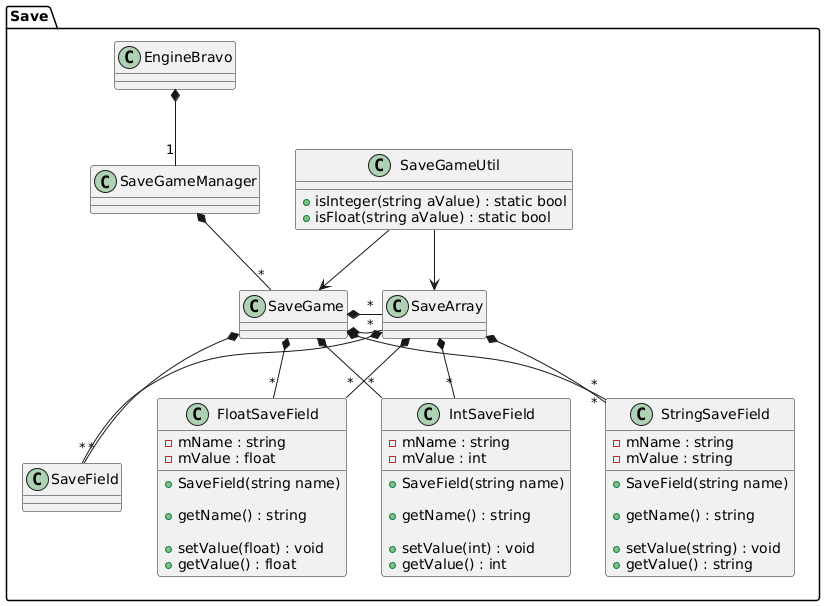
\includegraphics[width=\textwidth]{savegames.png}
The savegame system is largely similar to its equivalent in Unity.
The three data types which can be stored are represented by separate classes.
This way, the user does never need to manually check for types before retrieving the data.

\section{Networking}
The engine will support multiplayer.
As the customer wants the engine to follow the Unity engine API, the multiplayer system wil follow the multiplayer package of unity \textbf{Netcode}.

\subsection{Network library}
Multiple libraries have been considered, for example ENet, RakNet or Boost.
The uses library is SLikeNet. This library is a continuation of RakNet, which is a well known and well documented library.
The library is also easy to use and has a lot of features that are useful for the engine.

\subsection{Class diagram}

\begin{figure}[H]
    \centering
    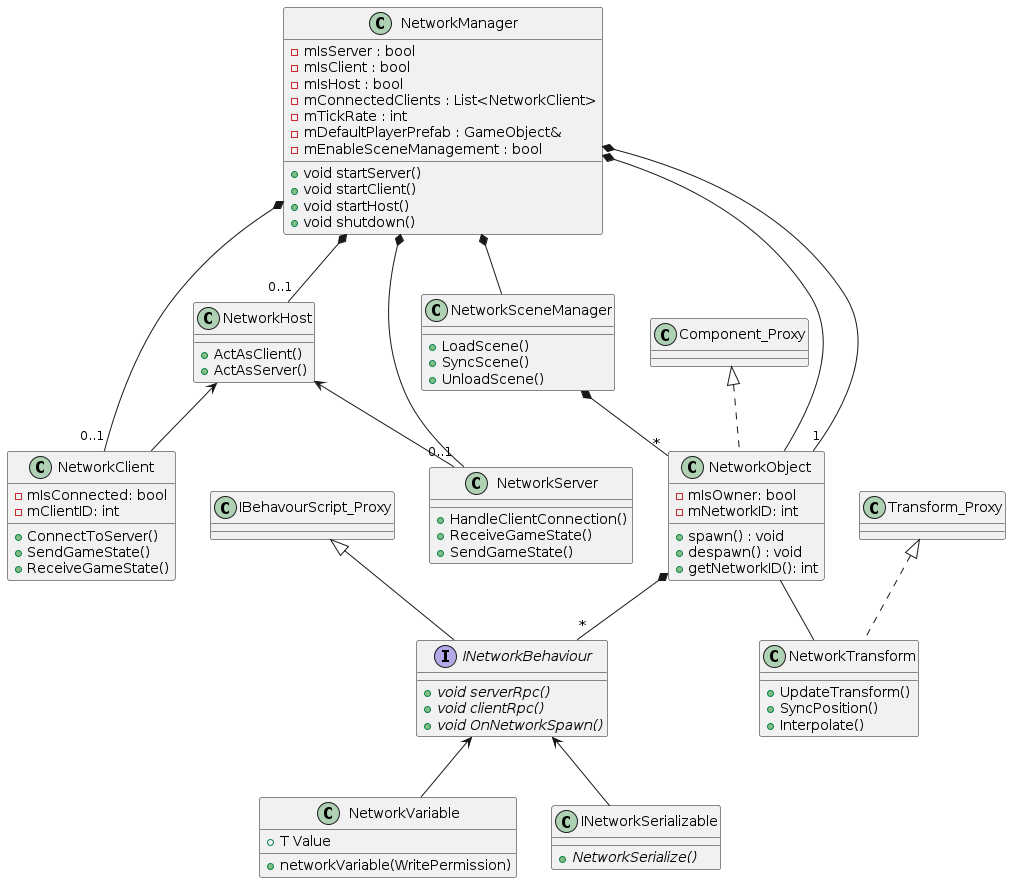
\includegraphics[width=\textwidth]{networkingClassDiagram.png}
    \caption{class diagram of the networking system}
    \label{fig:networkingClassDiagram}
\end{figure}
In figure \ref{fig:networkingClassDiagram} the proxy classes are classes that are defined in a different class diagram.

A central manager named NetworkManager is used to manage the networking features.
An application can either be a server, a client or both and is then named a host.
To send information over the network a NetworkObject is used.
This object inherits Component class and can be added to a GameObject to define that this object can be sent over the network.
NetworkBehaviour inherits the behaviour class and can be used to send specific information over the network.
The NetworkTransform is used as a standard implemenation of sending the transform information over the network.
If a game programmer wants more control of what information is send when it should send this information with the NetworkBehaviour.

To send information over the network a NetworkVariable must be used.
This is a template class that defines information and how that information can be serialized.

\section{Multithreading}
Multithreading is not added to the engine as it lies out of the scope of the project.

\end{document}
